\newpage
\section{Problem 2: Rainbow color map}
This figure shows the world elevation found on \url{https://commons.wikimedia.org/wiki/File:Elevation.jpg}. This visualisation\'s purpose is to inform about to world height difference and may be aimed for people interested in typography, flight planing, mountain climbing. It does not fail to convey the information and shows a difference between the elevation due to the fact that its represents the height different with a texture and more warmer color. The rainbow color in this case does not represent a clear visualisation in my opinion. This is because the color red and green have no added value regarding the elevation difference. Furthermore in this case the map gives of a \'loud\' feeling.


\begin{figure}[!htb]
    \centering
    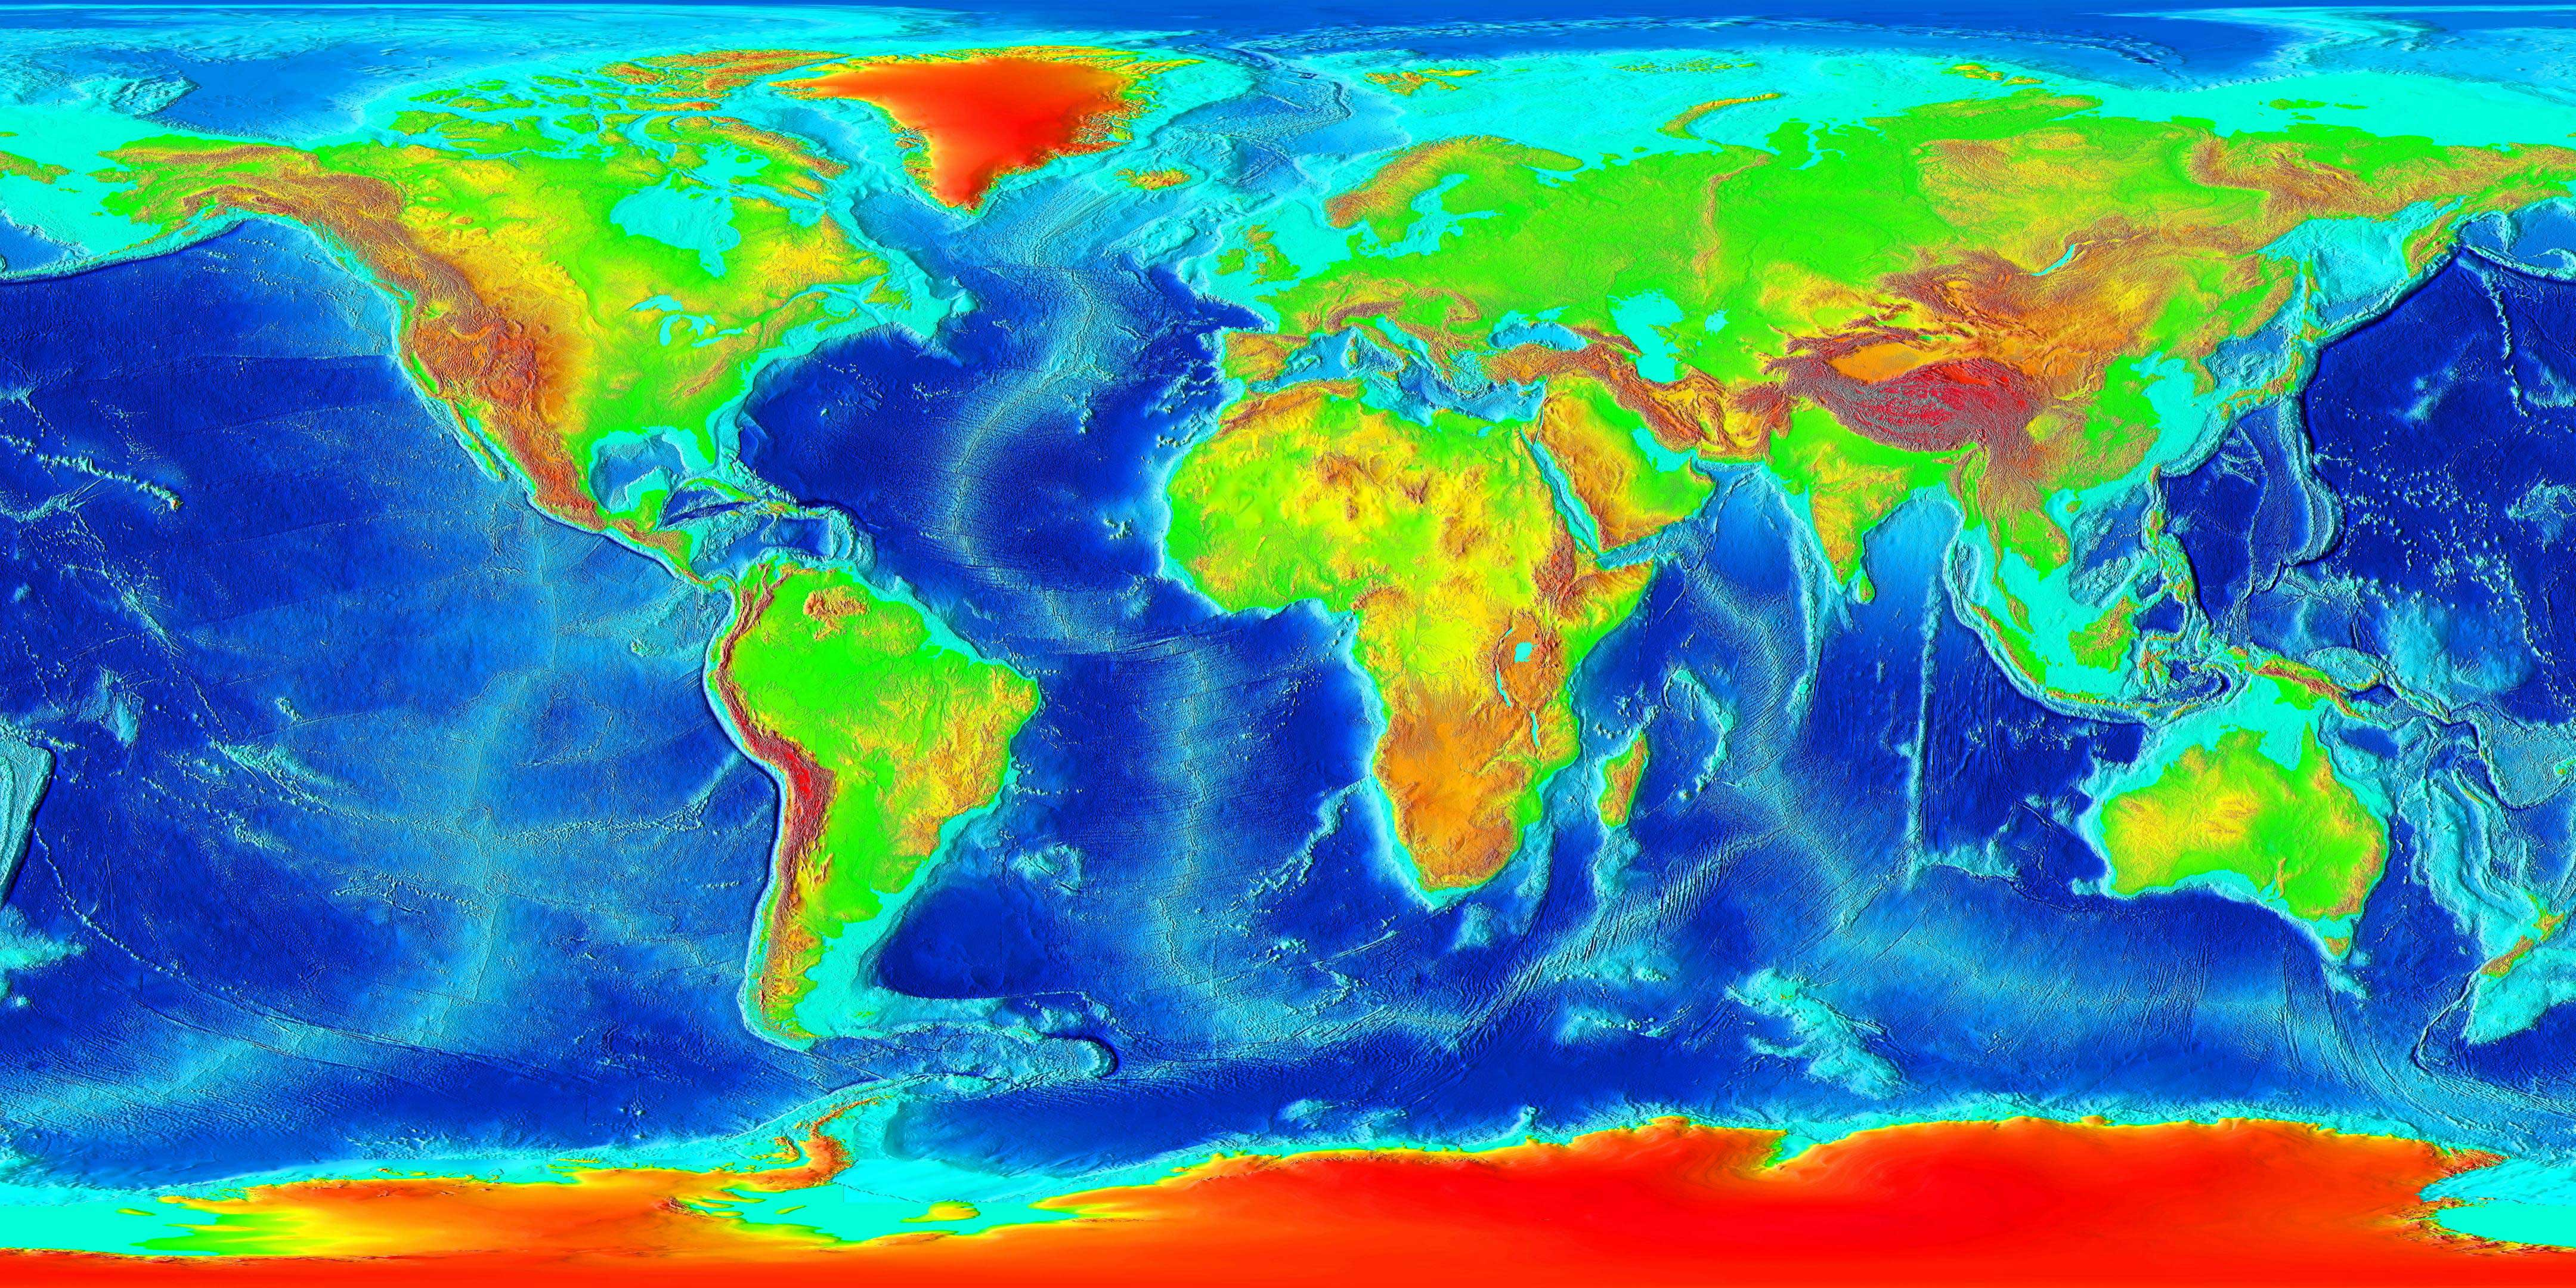
\includegraphics[width=\linewidth]{Figures/Elevation.jpg}
    \caption{World elevation map}
    \label{fig:elev}
\end{figure}